\chapter{Experimental setup}

\section{The track and the environment} \label{sec:track}
The track we used is called USI track, shown in Figure \ref{fig:usitrack}. It strongly resembles one used by \citet{DBLP:journals/corr/abs-2008-00715} in Learning to Drive. We do have a simulated version built in Unity and an actual printed track. The choice fell on this track since it is complete, it includes a straightaway, right turn, left turn, wide turn and very steep turn. Beside that, \citet{DBLP:journals/corr/abs-2008-00715} already proved that the agent can learn on this type of track and the focus of this thesis is more on replicating a real agent learning to self-drive in real world and not creating a new model with a particular feature.

\begin{figure}[h]
    \centering
\begin{minipage}{.5\textwidth}
    \centering
    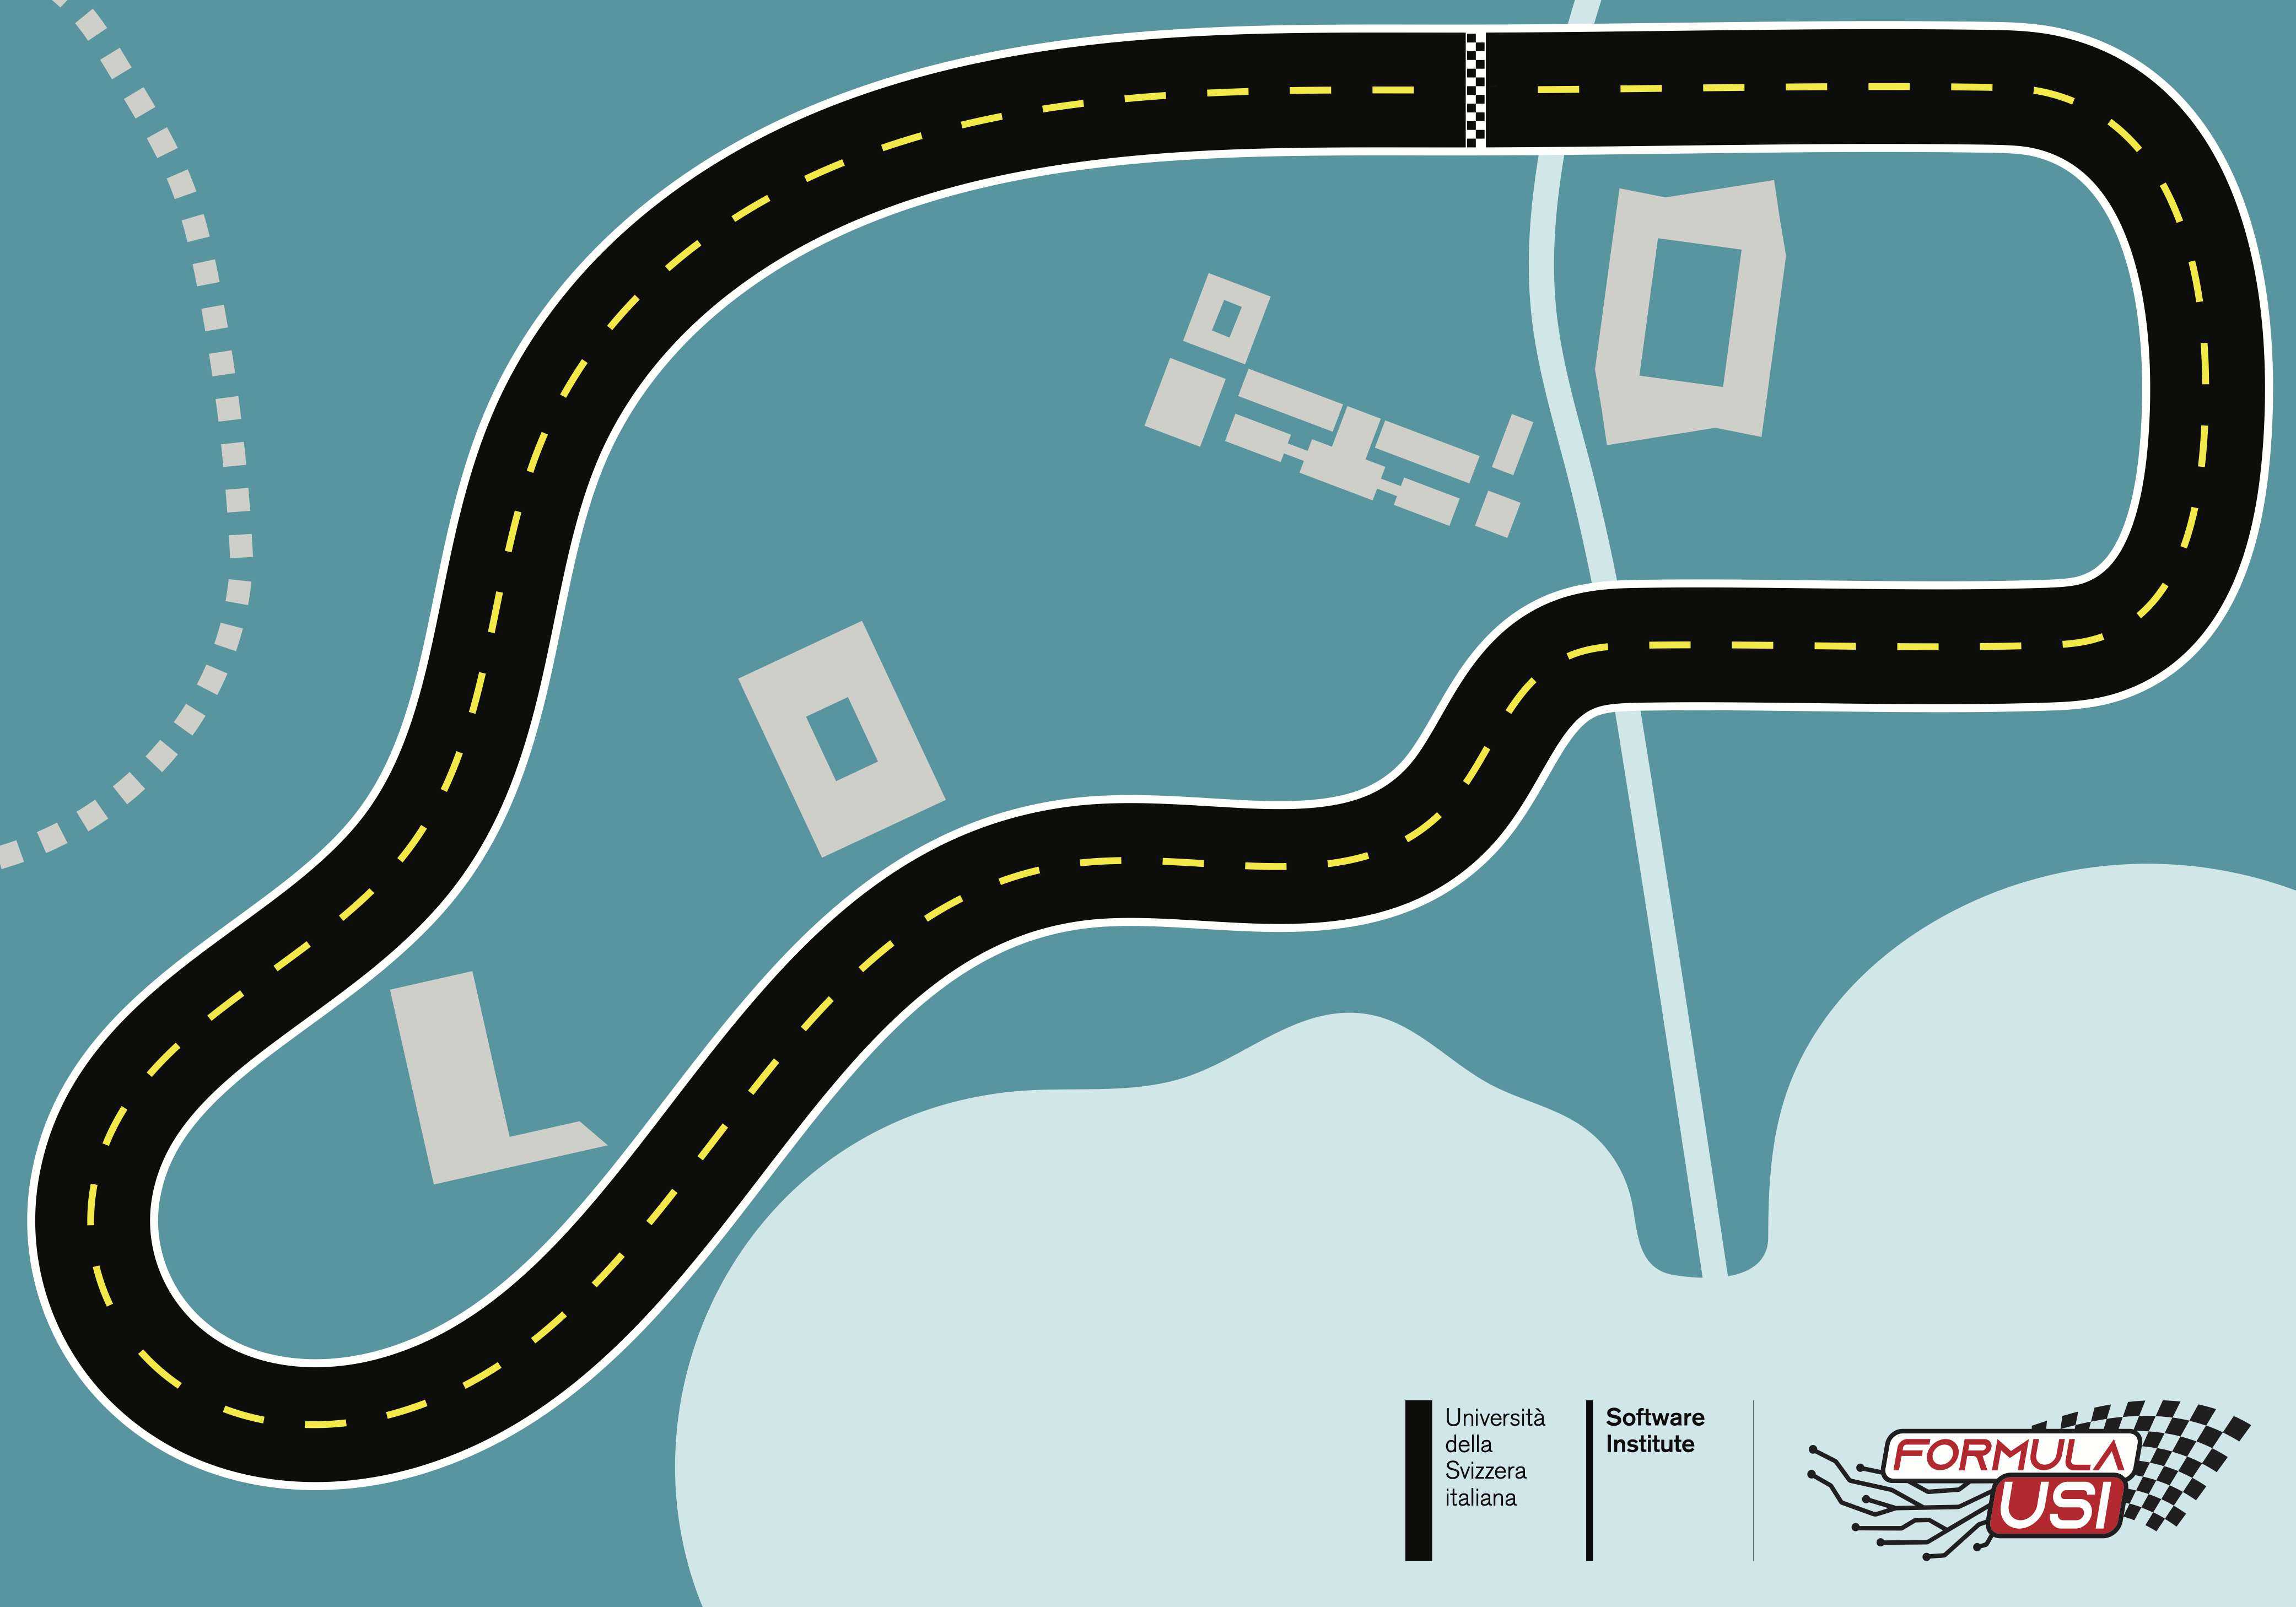
\includegraphics[width=0.85\textwidth]{setup/usi_track_real.png}
    \captionof{figure}{Real USI track TODO}
    \label{fig:usitrack}
\end{minipage}%
\begin{minipage}{.5\textwidth}
    \centering
    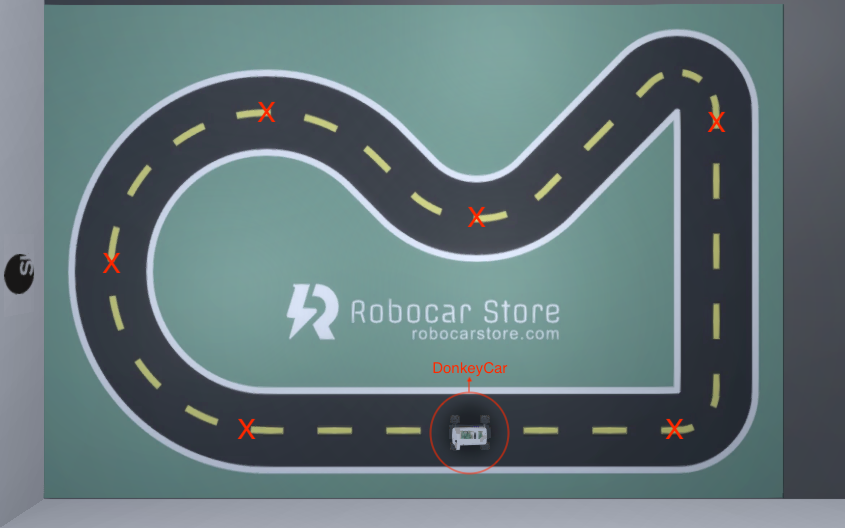
\includegraphics[width=0.95\textwidth]{setup/usi_track.png}
    \captionof{figure}{Simulated USI track}
    \label{fig:usitracksim}
\end{minipage}
\end{figure}

The learning of the agent, as shown later on, is straightforward, except the very steep turn which is considerably harder than the others. This difficulty is due to the limited steering angle of the robot and in the real world the aforementioned adversity is even more marked as well see. 

The default starting line in both tracks is where the Donkey is placed in Figure \ref{fig:usitracksim}. Certainly, in the real track it is an imaginary line that we use as a starting point and of course the laying of the car at each episode beginning cannot be exact but approximate. Beside that, there are a few checkpoints, approximately highlighted with a cross in Figure \ref{fig:usitracksim}, troughout the track that can be used as starting points depending on the learning strategy chosen. The simulator provides the following possibilities:

\begin{itemize}
    \item \textbf{Start:} The episode start always at the starting line.
    \item \textbf{Checkpoint:} The episode start at the latest checkpoint reached during the previous episode.
    \item \textbf{All:} All the checkpoints are used cyclically starting from the starting line and proceeding one by one forward for each episode.
    \item \textbf{Random: } The starting point is chosen randomly, between the available checkpoints, at the beginning of each episode.
\end{itemize}
Furthermore, the simulator let us choose where a lap ends. It can end where the DonkeyCar started or at the starting line.

%TODO: AGGIUNGI referenza punti di partenza.

\section{DonkeyCar}

The real Remote Controlled DonkeyCar is essentially a standard DonkeyCar as described in Section \label{sec:donkeycar}. To recap it is a remote controlled car equipped with a microcontroller NVIDIA Netson Nano and a camera sensor. The RGB pictures are taken at a resolution of $320x240$ and at $20hz$ (20 frames per second), which means the algorithm must finish all iteration steps within $0,05$ seconds otherwise it would skip some frames and the learning or the driving may be compromised by the agent's non-responsiveness. This limitation is present only in real world since the simulator time can be slowed down to meet the needs. In our setting we have a standard 3 cell LiPO battery of 11.1V and 2200 mAh to power just the motors and the controller. During the training in the real world we often noticed a slow regression in term of speeds of the car, iteration after iteration. However, this problem can be solved by disconnecting the LiPO battery for a moment from time to time to restore full speed, which is why we suspect this problem may be caused by the battery. Furthermore, an external power bank with 10000mAh/37Wh of capacity and an output of 5V and 2.4A powers the Jetson Nano which with this capacity, is more than enough to overcome the longevity of the LiPO battery.

\section{Training modality}

\subsection{Simulation}\label{subsec:sim}
In simulation, the training of the agent is straightforward since all the operation are done on the host machine, moreover it is not required a GPU machine to accomplish all the steps in time, at least until the cyclegan is introduced. Even though an on-policy RL algorithm could be implemented, an off-policy algorithm is chosen since in real world, in our setting, the on-policy method is not replicable given the limited computational power of the microcontroller. Beside that, we want to compare the same type of algorithm in the two type of environments. In pratice, a pretrained AE/VAE provides a representation of the state in the form of a latent vector, the agent drives with a policy kept constant during the episode and all the frames and actions are collected into a buffer. When the simulator reports that the car has crashed or went out of track more than a predefined distance, the episode terminates. The episode ends also when the car has reached the starting point or, in our setup, it reaches 1000 steps. Finally, at the end of the episode, a policy is trained using the collected buffer and the new parameters are used to update the driving policy.

\subsection{Real world} \label{subsec:real}
Since the microcontroller equipped by the DonkeyCar is a low capability calculator, a few precautions need to be taken in order to to train the agent. Firstly, as mentioned above, an off-policy method like SAC allows to relocate the actual training, and consequently the very expensive gradient back-propagation, to another machine with more resources. Secondly, the use of representation learning (AE/VAE) allows to reduce significantly the size of the RL neural networks and moreover the pre-training of the encoder can be done in advance on the host machine speeding up the process. In practice the functioning is similar to the one seen in previous Section \ref{subsec:sim}. The microcontroller operates the driving policy, collect the image, forward it through the AE/VAE, then the agent chose an action based on that representation. This process is repated until a human supervisor ends the episode for the car gone off the track. The episode also terminates when the DonkeyCar reaches, in our setup, 1000 steps. Hereafter, all the steps information, like latents vectors, actions and rewards are collected into a buffer up to a predefined size and are sent through the network to the host calculator that actually train the policy at the end of the episode. After the training, the new parameters are sent back to the DonkeyCar and the process is repeated until convergence.

\section{Communication - MQTT}

As described in Section \ref{subsec:real}, when training in real world, the host machine and the DonkeyCar must communicate wirelessly multiple times during the training. MQ Telemetry Transport (MQTT) is the most used messaging protocol for the Internet of Things (IoT). It includes all the rules that define how devices can write (publish) and read (subscribe) data over the internet. The sender (Publisher) and the receiver (Subscriber) communicate via topic and are decoupled from each other. The connection between them is handled by an MQTT broker that filters all incoming messages and distributes them correctly to the Subscribers of the topic. In pratice any device can publish a message on a topic, then the broker take care of dispatching it to subscribers of that topic. In particular we used the HiveMQ broker that allows the connection of up to 100 clients with no cost. The topics defined to manage the communication between the host machine and the DonkeyCar are:

\begin{itemize}
    \item \textbf{Stop car:} The host machine writes a signal on this topic, that is constantly monitorated by the DonkeyCar, to inform that the episode must terminate.
    \item \textbf{Replay buffer:} Once the episode terminate, all the collected information by the DonkeyCar are sent to the host machine through this topic.
    \item \textbf{Replay buffer received:} The host machine uses this topic to acknowledge DonkeyCar that it has received the buffer.
    \item \textbf{Parameters:} Once the training is complete, the host machine sent the updated neural network parameters through this topic.
    \item \textbf{Start episode:} The host machine uses this topic to acknowledge DonkeyCar that a new episode can start.
    \item \textbf{Speed modifier:} This topic can be used by the host machine to inform the DonkeyCar that it must change its throttle by the sent value that can be either positive or negative.
\end{itemize}

Notice that this protocol is not complety reliable so some precautions and check must be done when implenting it, especially in real-time system where some actions cannot be delayed.

\section{Dataset}
With regard to the dataset we need to define two types of dataset. A dataset composed of images collected on the simulator to train the relative autoencoder and after that the simulated RL agent, and a similar one composed of real images collected on the printed track. A few example of each one are respectively shown in Figures \ref{fig:datasetsim} and \ref{fig:datasetreal}.

\begin{figure}[h]
    \begin{minipage}{.33\textwidth}
      \centering
      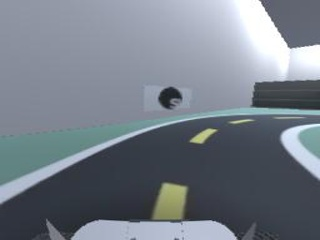
\includegraphics[width=0.95\textwidth]{setup/s1.jpg}
    \end{minipage}%
    \begin{minipage}{.33\textwidth}
        \centering
        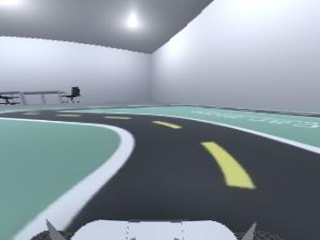
\includegraphics[width=0.95\textwidth]{setup/s2.jpg}
    \end{minipage}%
    \begin{minipage}{.33\textwidth}
        \centering
        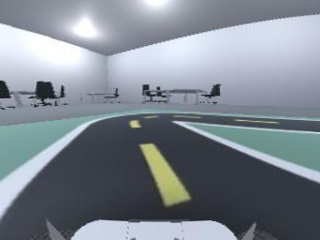
\includegraphics[width=0.95\textwidth]{setup/s3.jpg}
    \end{minipage}
    \captionof{figure}{Images extracted from the simulated dataset}
    \label{fig:datasetsim}
  \end{figure}

\begin{figure}[h]
\begin{minipage}{.33\textwidth}
    \centering
    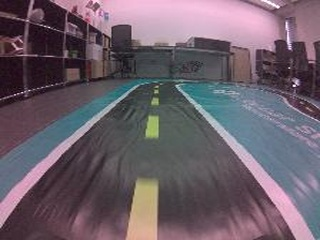
\includegraphics[width=0.95\textwidth]{setup/r1.jpg}
\end{minipage}%
\begin{minipage}{.33\textwidth}
    \centering
    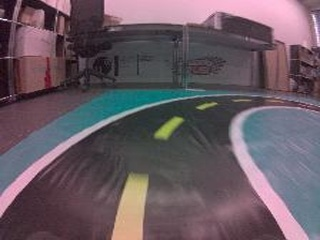
\includegraphics[width=0.95\textwidth]{setup/r2.jpg}
\end{minipage}%
\begin{minipage}{.33\textwidth}
    \centering
    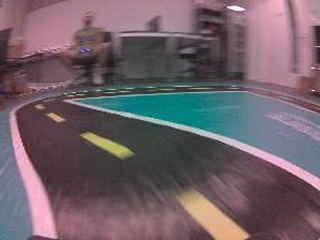
\includegraphics[width=0.95\textwidth]{setup/r3.jpg}
\end{minipage}
\captionof{figure}{Images extracted from the real dataset}
\label{fig:datasetreal}
\end{figure}

During the experiments resulted that a dateset of $\sim 10000$ pictures was enough to reach our goals, furthermore notice that smaller datasets may not be sufficient for the encoder to learn a good representation. To collect each of the datasets are enough $\sim10$ minutes if we run the algorithm at $20hz$ (20 frames per second) as we did. Beside that, all the pictures from the real world must be collected with a certain environmental condition that should remain consistent in time, also during the training of the agent to avoid problems. In our case, it was collected with all windows closed and the with maximum light to make it easy to be replicated. 

Since we want our RL agent to focus exclusively on the track we found convinient to crop the top 100 rows of each pictures to remove the background, and to reduce the complexity of our algorithm, we downscale each images from $320x140$ to $160x80$ before feeding them to the encoder. The resulting pictures are shown in Figures \ref{fig:datasetsimcropped} and \ref{fig:datasetrealcropped}. Note that during training, the training set is split in validation and training set with a ratio $20/80$ and the test set is collected apart and consist of $\sim 1000$ images for each dataset.

\begin{figure}[h]
    \begin{minipage}{.33\textwidth}
      \centering
      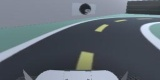
\includegraphics[width=0.95\textwidth]{setup/cs1.jpg}
    \end{minipage}%
    \begin{minipage}{.33\textwidth}
        \centering
        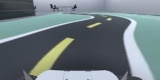
\includegraphics[width=0.95\textwidth]{setup/cs2.jpg}
    \end{minipage}%
    \begin{minipage}{.33\textwidth}
        \centering
        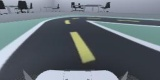
\includegraphics[width=0.95\textwidth]{setup/cs3.jpg}
    \end{minipage}
    \captionof{figure}{Examples of cropped simulated images}
    \label{fig:datasetsimcropped}
\end{figure}

\begin{figure}[h]
\begin{minipage}{.33\textwidth}
    \centering
    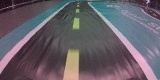
\includegraphics[width=0.95\textwidth]{setup/cr1.jpg}
\end{minipage}%
\begin{minipage}{.33\textwidth}
    \centering
    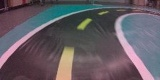
\includegraphics[width=0.95\textwidth]{setup/cr2.jpg}
\end{minipage}%
\begin{minipage}{.33\textwidth}
    \centering
    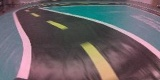
\includegraphics[width=0.95\textwidth]{setup/cr3.jpg}
\end{minipage}
\captionof{figure}{Examples of cropped real images}
\label{fig:datasetrealcropped}
\end{figure}
Finally, for the cyclegan, the dataset can be even smaller $\sim 5000$ pictures for both real and simulation. No crop is applied and a resize to $256x256$ pixels is done to match the network size provided by \citet{CycleGAN2017}. And the test sets match the ones used for the encoders. After applying the cyclegan in our experiments, the pictures are reshaped and cropped to match the need of the autoencoder.